\section{Evaluation}%
\label{section-evaluation}

In this section we evaluate our debugger to assess the efficacy of our
approach, by answering RQ3.  We want to compare the original situation
with the situation when using RxFiddle.  RxFiddle is our ``treatment''
for the RP debugging problem, so we use an experiment, in which we
control for the debugger that subjects use, to test our hypothesis that
RxFiddle improves debugging.

Ko et al.~\cite{ko2015practical} describes two commonly used measures
for experiments regarding tools in Software Engineering:  \emph{success}
on task, and \emph{time} on task.  The goal of our experiment is to
measure the \textit{time} required to solve programming problems
correctly.  If our reasoning for RQ2 is right and our design leans
itself for RP, we expect to see that the group using RxFiddle can more
quickly reason about the reactive code at hand and can trace bugs
faster.  We do not choose only success or correctness as a measure for
the experiment, as we expect both groups to be able to complete the
tasks correctly:  while the current debugging situation is non-optimal,
it is still used in practice, indicating that it works at least to some
extend.  The construct of time also matches debugging better; a
developer needs to continue debugging \textit{until} he finds an
explanation or a solution to his problem, and incorrect assumptions can
be tested and corrected.

We measure the time from the moment the participant receives the
question until the correct answer is given.  Participants use either the
built-in Chrome Browser debugger (group \emph{Console}) or - the
treatment - our RxFiddle debugger (group \emph{RxFiddle}).  This single
alternative Console debugger together with the experiment UI (which acts
as a small IDE) offers all the debugging capabilities subjects of our
preliminary interviews (RQ1) reported to use.

The experiment consists of a questionnaire, a warm-up task and four
programming tasks, all available in a single in-browser application, of
which the source code is available at~\cite{rxfiddle-doi}.  The
questionnaire contains questions regarding age, experience in several
programming languages and several reactive programming frameworks.  We
use this self estimation as a measurement of skill instead of a pretest,
since it is a faster and better estimator~\cite{kleinschmager2011rate,feigenspan2012measuring,siegmund2014measuring}.
The warm-up program is situated in the same environment as the
programming problems and contains several tasks designed to let the
participants use every control of this test environment.  The first two
programming problems require the participants to obtain an understanding
about the behavior of the program and report the findings.  The last two
programming problems contain a program with a bug.  The participants are
asked to find the event that leads to the bug in the third problem and
to identify and textually propose a solution in the fourth problem.  The
first two problems are synthetic examples of two simple data flows,
while the latter contain some mocked (otherwise remote) service which
behaves like a real world example.

We use a between-subjects design for our setup.  While this complicates
the results - subjects have different experience and skills - we can not
use a within-subjects design as it would be impossible to control for
the learning effect incurred when asking subjects to perform survey
questions with and without the tool.  This also allows us to restrict
the amount of tasks to incorporate in the experiment, requiring less
time from our busy subjects.  In the experiment environment subjects can
answer the question and then hit ``Submit''; alternatively they can
``Pass'' if they do not know the answer.

\subsection{Context} The experiment was run both in a offline and in an
online setting.  The offline experiment was conducted at a Dutch
software engineering company.  Subjects are developers with several
years of programming experience, and range from little to no experience
with RP to many years of experience (Figure%
\ref{fig-experience}).  As we do not try to measure the effect of
learning a new tool, but rather using a tool after learning to use it,
we explained RxFiddle in the introductory talk and added the warm-up
question to get every participant to a minimum amount of knowledge about
the debugger at hand.

The online experiment was announced by the authors on Twitter, and
consequently retweeted by several core contributors to RP libraries, and
via various other communication channels, such as Rx related Slack and
Gitter topics.  Subjects to the online experiment took the test at their
own preferred location and have possibly very different backgrounds.
Several short video tutorials were created and included in the online
experiment to introduce the participants to the debug tool available to
them and the tasks they needed to fulfill.  The introductory talk was
used as the script for the videos, in order to get all participants to
the same minimum level of understanding.

\begin{figure}[t]
    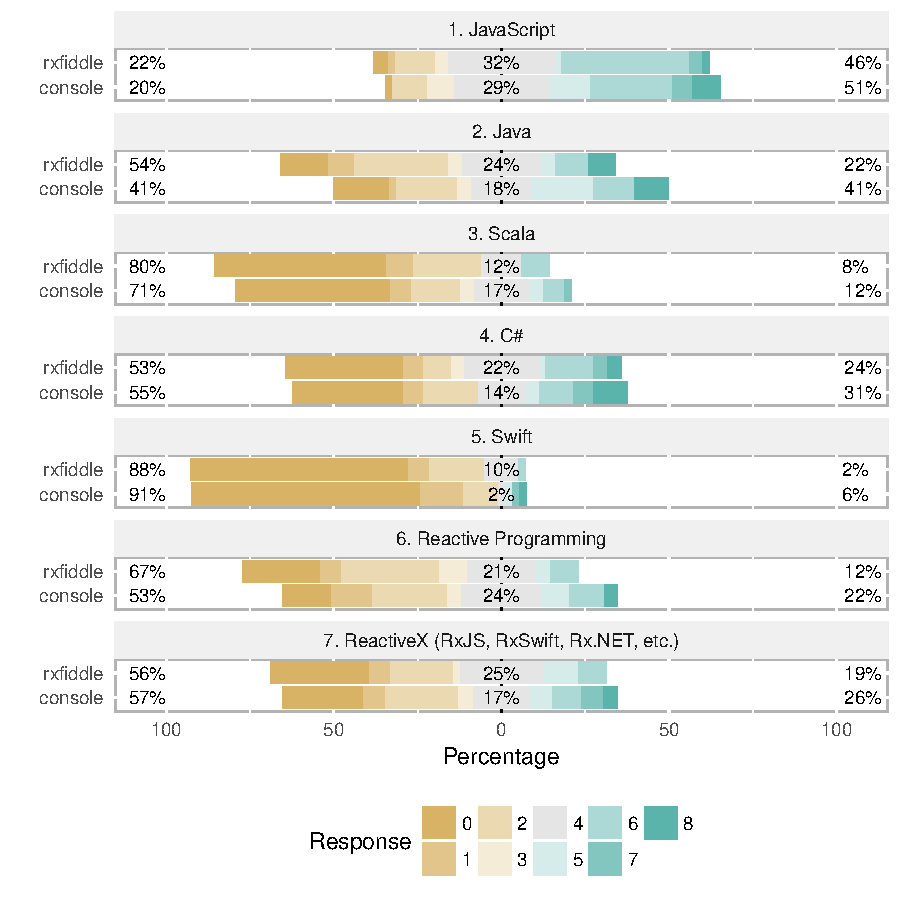
\includegraphics[width=\columnwidth]{images/experience.pdf}
    \caption{Experience in various programming languages, 9-point Likert
    scale (0 = none, 2 = beginner, 4 = medium, 6 = senior, 8 = expert)}%
    \label{fig-experience}
\end{figure}
